\documentclass[a4paper,12pt]{scrartcl}
\usepackage[utf8]{inputenc}
\usepackage[french]{babel}
\usepackage[T1]{fontenc}
\usepackage{amsmath}
\usepackage{color}
\usepackage{graphicx}
\usepackage{isotope}
\usepackage{float}
\usepackage{scrpage2}
\usepackage{vanadin}
  

\title{Résonance magnétique nucléaire (RMN) du \isotope[13]{C} haute résolution en phase solide}
\subtitle{TP Cesire}
\author{Mona Dentler,\\ Sabine Engelhardt et Laura Hilpert}
\publishers{Université Joseph Fourier, CEA Grenoble}

 \begin{document}

 \pagestyle{empty}
 \begin{center}
  \makeatletter
   %\titlefont
  \@subject
  \vspace{2cm}

  \Huge
  Résonance magnétique nucléaire (RMN) du \isotope[13]{C} haute résolution en phase solide\newline
  \Large TP Cesire
  \vspace{1cm}

  \@author
  \newline\empty\\
  \@publishers


  \@date
  \makeatother
 \end{center}
 \vfill

 \begin{abstract}
  Le but de ce TP Cesire est de comprendre comment faire spectre des solides à l'aide d'une RMN. On le sait déjà très bien faire pour une solution, mais pour un solide il y a quelques problèmes. Un solide est inhomogène et il y a la force dipôlaire qui dérange la mesure, car les atomes sont fortement couplés. En solution cette force se moyenne à zéro.\\ 
  Comment alors obtenir un bon spectre d'un solide? D'abord nous avons appris un peu de la théorie d'une RMN et surtout les solutions pour faire une RMN d'un solide pour ensuite les vérifier en mesurant. 
 \end{abstract}
 \newpage
\pagestyle{scrheadings}
 \tableofcontents

 \section{Résonance Magnétique Nucléaire (RMN)}
  \subsection{Fonctionnement d'une RMN}
  La RMN use la résonance de spin des noyeaux atomiques. L'échantillon est mis dans un champ magnétique $B_0$ externe pour avoir les moments magnétiques des atomes paralell ou anti-paralell au $B_0$. Par conséquence le moment magnétique d'un atome tourne autour cette direction avec la fréquence de Larmor $\omega_L=\frac{\gamma}{2\pi}B_0$ avec $\gamma$ le rapport gyromagnétique. $\omega_L$ est specifique pour chaque materiél, à cause du moment angulaire de l'atome. Le champ magnétique est donc augmenté dans cette direction, mais cette augmentataion est à peine mesurable, alors on use une autre méthode.\\
  Une onde électro-magnétique (em) avec la fréquence $\omega_L$ en grandeur des ondes radio est envoyé à l'échantillon. Les moments magnétiques commencent à basculer car l'onde em leurs donne l'énergie qui est necessaire. Normalement on arrêt l'onde quand les spins sont à \unit[90]{\degree} par rapport au $B_o$. Dans cette direction on peut mesurer le champ magnétique $M$ causé par les moments magnétique qui est perpendiculaire au $B_0$.\\
  Si on arrête l'onde em les moments magnétique se remettent en position originale. Cette relaxation est dû à l'interaction spin-spin et à l'interaction de spin-atome. Le temps de relaxation est différent pour chaque matériel et en mesurant le changement de $M$ on peut y déduire le temps de relaxation.   \newline
  La sensibilité d'une RMN est 
  \begin{equation*}
   \frac{N_{\alpha}}{N_{\beta}}=\exp\left(-\frac{\Delta E}{k\cdot T} \right)=\exp\left(-\frac{\text{h}\nu}{kT}\right)\propto B_0
  \end{equation*}
  donc proportionel à la grandeur de $B_0$ et antiproportionel à la température de l'échantillon.\newline
  L'atome le plus simple de détecter est l'Hydrogène H. Cet atome a un moment magnétique très fort et donc il est facile à tourné par l'onde em.

  \subsection{RMN d'une solution}
   Avec cette dispositif on peut faire un spectre très précise d'une solution. Une solution est isotrope donc il n'y a pas des interactions qui dérange la mesure. On obtient des spectre avec des pics trés précis et grand.

  \subsection{Problématique d'un RMN d'un solide}
   Si on essaie de faire un spectre avec ce dispositif, on ne voit qu'un ou plusieurs signaux très large et de faible hauteur. Avec ce dipositif la distinction entre les atomes ou plutôt les raies du spectre des différents élemente n'est plus possible. Ce chevauchement est provoqué par le déplacement chimique causé par les électrons des cortège électronique d'un datome et par les interactions dipolaires. En plus un solide est anisotrope donc à chaque l'angle on trouve un autre ordre des atomes. Un autre problème c'est la couplage dipolaire entre les atomes qui provoque une relaxation assez vite qui est difficile à mesurer.\\
   La temps de mesure augment car le \isotope[13]{C} n'est pas très sensible, par conséquence on a besoin d'une onde em plus longue pour basculer le moment magnétique du \isotope[13]{C}.

  \subsection{Solutions}
   Car nous avons fait des RMN du \isotope[13]{C}, nous présontons les solution pour cet isotope. Il y a trois aspects différents:
   \begin{enumerate}
    \item La découplage dipolaire pour élimiter les interactions dipolaires.
    \item La rotation à l'angle magique pour éviter l'anisotropie.
    \item La polarisation croisée pour augmenter la sensibilité du \isotope[13]{C}.
   \end{enumerate}

   \subsubsection{Découplage dipolaire}
    Le champ effectif pour le spin d'un atome est
    \begin{equation*}
     B_{eff}=B_0 + B_{couplage} 
    \end{equation*}
    avec $B_{couplage}$ le champ local autour d'atome causé par les interactions dipolaire et scalaires entre les atomes. Par une onde em de haute puissance les couplages entre H et \isotope[13]{C} sont éliminés car l'H est plus sensible que le \isotope[13]{C} et on se  débarasse de l'aimantation $H$ d'H. La découplage est très important pendant le temps de mesure la relaxation de \isotope[13]{C}. On peut aussi applicer une impulsion de \unit[90]{\degree} et ensuite changer la phase de l'onde par $\nicefrac{\pi}{2}$ pour garder le moment magnétique perpendiculaire d'H (spin-lock), alors le couplage dipolaire est éliminé. 

   \subsubsection{Rotation de l'angle magique}
    On trouve pour l'aimantation
    \begin{eqnarray*}
     H_{\sigma}&=&\hbar H_0\gamma I_z\left(\frac{1}{2}\sin\left(2\alpha\right)\text{tr}\left(\sigma\right)+\frac{1}{2}\left(3\cos^2\alpha-1\right)\sum_i\sigma_i\sin^2\beta_i\cdot\cos\left(2\left(\omega_r t+\Phi_i\right)\right)\right)\\
     H_{\sigma}\left(t\right)&=&\hbar H_0\gamma I_z\left(\frac{1}{2}\sin\left(2\alpha\right)\sum_i\sigma_i\sin\left(2\beta_i\right)\cos\left(\omega_r t+\Phi_i\right)+\frac{1}{2}\sin^2\alpha \sum_i\sigma_i\sin^2\beta_i\cdot\cos\left(2\left(\omega_r t+\Phi_i\right)\right)\right)
    \end{eqnarray*}
    Avec $\alpha=\unit[54,7]{\degree}$ donc $3\cos^2\alpha-1=0$ entre l'échantillon et $B_0$ on se débarasse du second terme de la première équation. C'est à dire que les interactions dipolaires et quadrupolaire et l'effet de l'anisotropie de déplacement chimique sont éliminés. Une rotation suffisamment vite elimine la dépendance du temps du deuxième équation. Avec une rotation trop lente il y a plusieurs raies avec une distance égale à la vitesse de la rotation. Le raie le plus grand n'doit pas être celui du vrai signal. 

   \subsubsection{Polarisation croisée}
    Pour diminuer la temps de mesure on transmet les moments magnétiques des H aux \isotope[13]{C}. Une impulsion de \unit[90]{\degree} bascule le moment magnétique d'H et après le spin-lock le fixe pour un certain temps. Avec la condition de Hartman-Hahn
    \begin{eqnarray*}
     \omega_C=\omega_H\\
     \Rightarrow \gamma_c H_C=\gamma_H H_H
    \end{eqnarray*}
    le moment magnétique est transferé. Le temps de contact pendant laquelle on met la condition Hartman-Hahn doit être ni trop court ni trop long pour obtenir l'aimantation la plus grande pour le \isotope[13]{C}. 
    \begin{figure}[H]
     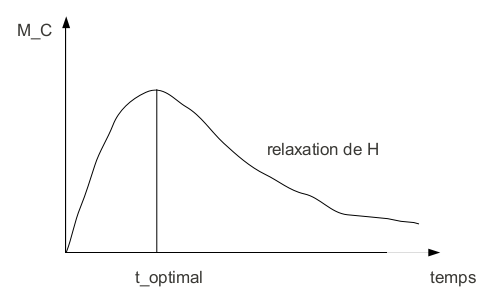
\includegraphics[width=0.6\textwidth]{bilder/schema_pol.png}
     \caption{Aimantation de \isotope[13]{C} en fonction de la temps de contact}
    \end{figure}
    Après quelque temps l'H se relaxe et donc l'aimantation de \isotope[13]{C} se diminue car moins d'aimantation est transmit et le \isotope[13]{C} se relaxe à son tour.
     

 \section{Dispositif expérimental}
  \subsection{Montage expérimental}
   Nous avons usé deux différents dispositifs experimentals, leur seule différence est que celui pour la mesure de la cellulose donne la possibilité des mesures plus précises.

   Le dispositif se constiste d'un électroaimant pour le champ magnétique exterieur dans lequel se trouve l'échantillon. L'échantillon est mis dans un petit roteur avec peu d'air pour ne pas déranger la mesure. Ce roteur est placé dans la bobine qui se trouve à l'interieur refroidi du électroaimant. Cette bobine est émetteur et sonde des ondes radios en même temps. 

   On peut choisir la fréquence de la rotation et le reste de la mesure est dirigé par l'ordinateur. Les dates sont directement transferé à l'ordinateur pour donner la possibilté d'y faire une transformation Fourier des dates pour obtenir le spectre.

   Le deuxième dispositif donne la possibilité de mesurer plus précise à cause de deux choses:
   \begin{itemize}
    \item L'interieur est plus froid, donc il y a moins de dérangement
    \item La rotation est plus vite, alors la structure est plus homogène
   \end{itemize}


  \subsection{Préliminaire} 
   Pour voir que l'échatillon est bien placé et le dispositif est bien calibré il faut d'abord faire un \flqq wob\frqq. \c Ca veut dire qu'on regarde l'énergie absorbé en fonction de la fréquence. On connaît la fréquence des atomes de l'échantillon qui on veut mesurer, ici nous avons usé la fréquence pour le \isotope[13]{C} et la fréquence pour le H. Cette fréquence est envoyé sur l'échantillon est on obeserve que le système absorbe l'énergie sauf à la fréquence ou on veut mesurer. 

   Si on ne fait pas cela avant la mesure on peut avoir deux choses qu'on ne veut pas. Premièrement on ne voit rien pendant la mesure car la réponse, donc la fréquence de la réponse, est absorbé et deuxièment ce qu'on veut surtout pas il y a la possibilité que l'énergie pas absorbée détruit la sonde, parce qu'elle est trop grande.

   \subsection{Influence des paramètres sur la mesure}
    \subsubsection{Nombre de scans}
     La différence signal/ bruit est proporionnel à $\sqrt{ns}$, donc pour améliorer le résultat par deux il faut avoir un nombre de scans $nd$ 4 fois plus grand.

    \subsubsection{Fréquence de la rotation}

    \subsubsection{Temps de contact}

    \subsubsection{Puissance des signaux}

 \section{Glycerine}
  Nous avons fait ces expériment pour verifier les différents théorie pour obtenir un beau spectre.

  \subsection{Rotation de l'angle magique}
   La première expérience était de changé la fréquence de la rotation de l'angle magique. On a dit que le solide semble plus homogène le plus vite il est tourné. Nous avons fait une mesure avec une rotation à \unit[4]{kHz}, puis \unit[3]{kHz}, \unit[2]{kHz}, \unit[1]{kHz}, \unit[0,75]{kHz}, \unit[0,5]{kHz},\unit[0,2]{kHz} et sans rotation. Dès la mesure de \unit[0,75]{kHz} nous avons augmenté le nombre de scans de 4 à 16 pour obtenir un meilleur spectre. 
   \begin{figure}[H]
    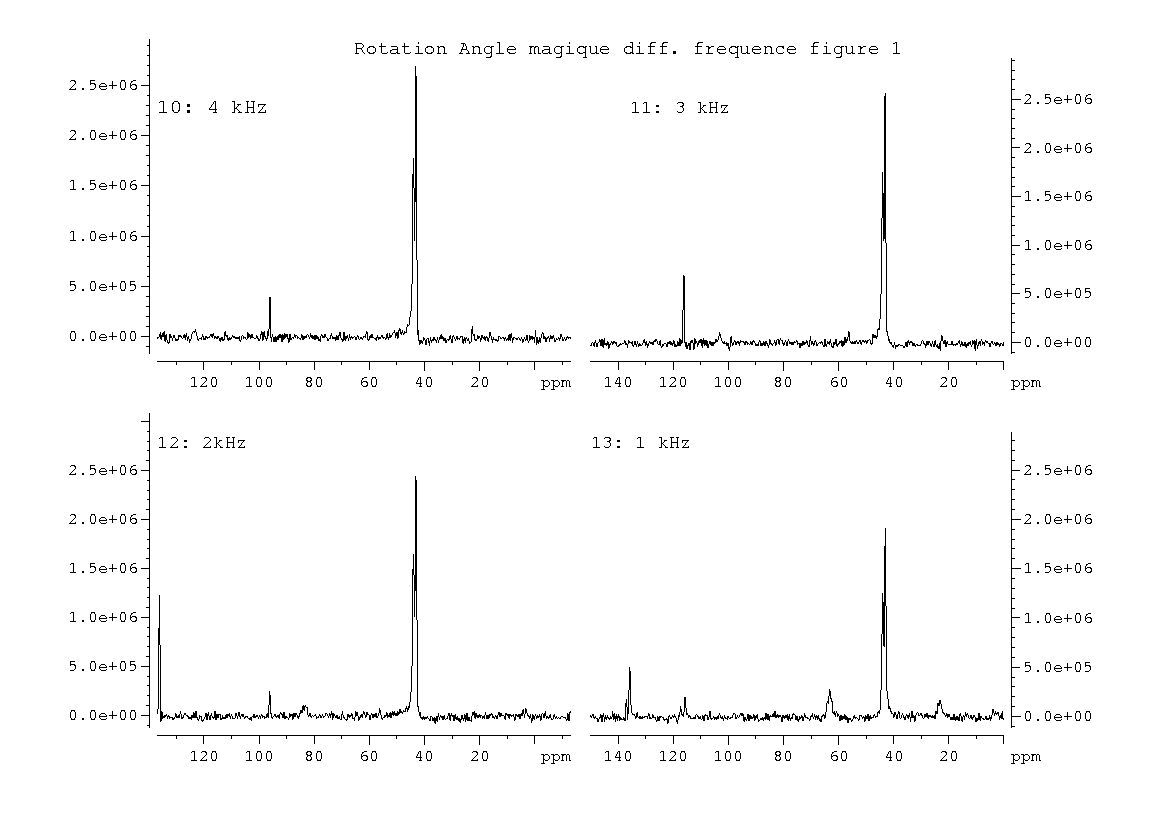
\includegraphics[width=\textwidth]{bilder/rotation.png}
    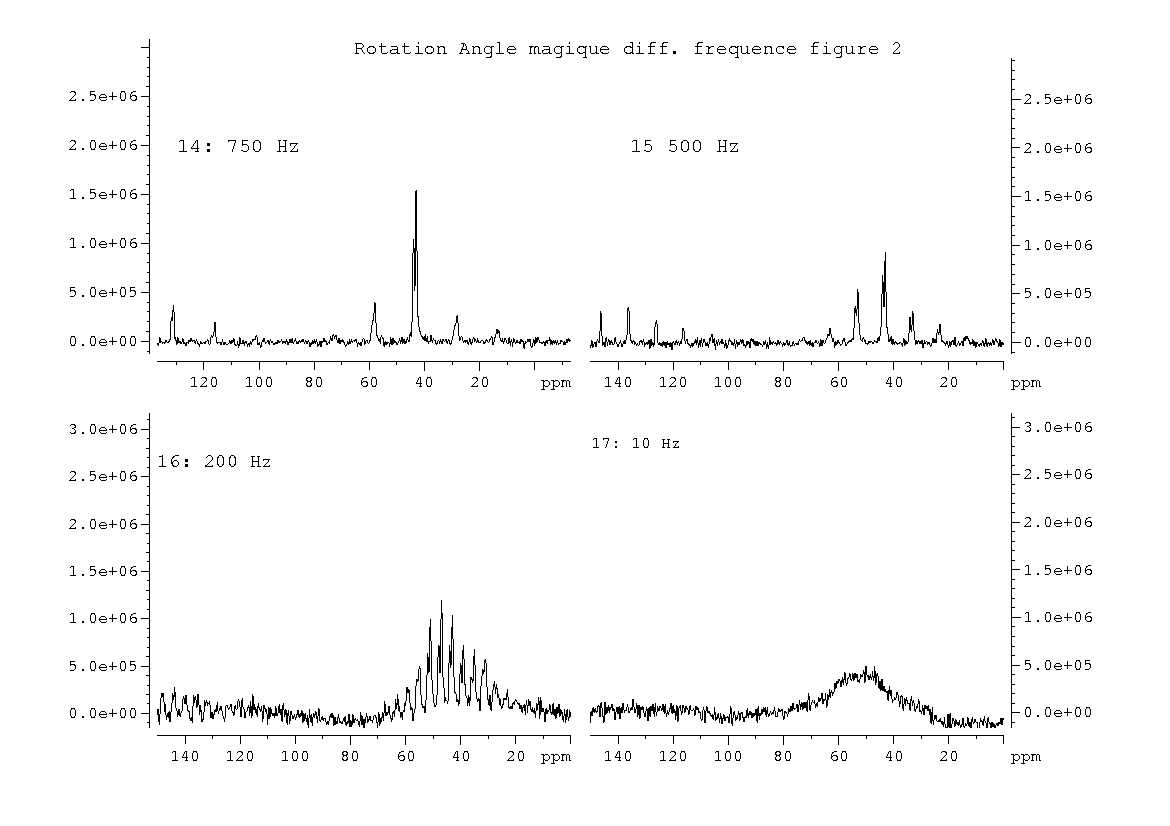
\includegraphics[width=\textwidth]{bilder/rotation2.png}
    \caption{\label{rotation}Les spectres pour les différents fréquences.}
   \end{figure}
   \paragraph{Interprétation}
    On voit bien dans les spectres de la figure \ref{rotation} à la p. \pageref{rotation} que les signaux qu'on veut obtenir se dimunue porportionnelement à la fréquence de la rotation. C'est à cause de la nombre de pics qui augmente. La mêmenombre de signaux est detéctés, mais il sont distribue sur différents pics. Dans le premier spectre avec \unit[4]{kHz} on ne voit que les deux pics fines assez grands de \todo{welche genau?} C et C. Dans le deuxième spectre on voit déjá plusieurs autres pics, les bandes rotationelles. On sait que ce sont des bandes rotationnelles car la distance entre le signal vraie et ses bandes rotationelles est $d=n\cdot f_{rot}$ avec $f_{rot}$ la fréquence de la rotation de l'angle magique. Dans le dernier spectre on ne voit rien. Il n' y a qu'un pic très large avec le maximum même pas à la position correcte. Le deuxième pic, le plus petit, n'est plus vue.

   \paragraph{Conclusion}
    Donc nous avons vu que c'est vraie quand diminue les artefacts causé par le déplacement chimique du solide avec la rotation de l'angle magique. 

  \subsection{Temps de contact}
   Le temps de contact c'est le temps pendant laquelle on transfere l'aimantation de \unit[90]{\degree} des atomes d'H aux atomes de C.

  \subsection{Puissance de Hartmann-Hahn}
 
 

 \section{Graines de salade}
  \subsection{Condition liquide}
 
  \subsection{CP masse}

  \subsection{DEPT ?}
   Spektrum mit gekippten Peaks, wenn an ungerader Anzahl von Protonen, irgenwie mit Kopplung

  \subsection{2D-Spektrum}
   wie Dept, aber Entkopplung glaube ich später
 
 

 \section{Cellulose}
  \subsection{Spectre \isotope[13]{C}}
   nicht erkennbar was was ist, am Ende Spektum nochmal zeigen +beschriftet  

  \subsection{Spectre H}
   Wasser peak und Artefakt, bandes rotationelles

  \subsection{Spin-diffusion}
  
  \subsection{Inadequate}

  \subsection{Hetcore}
 
   abgeschnitten Spinning sidebands, noch da fehler wegen zu kurz gemessen = Signal abgeschnitten
 
 

 \section{Conclusion}
 
 


\end{document}
